\section{Data Acquirer}\label{section:acquirers}

Data acquirer is a component downloading data from a social network (or any other component). Some social networks with free API impose limits on the amount of data downloaded (e.g., for Twitter limits refer to \footnote{https://developer.twitter.com/en/docs/basics/rate-limits}). These limits are tackled by downloading data continuously not in  one batch. 

The posts may come in various languages but the analyses can usually work only with English. For this reason, analysers can optionally translate all acquired posts from any language to English.

\subsection{Requirements and Dependencies}

\noindent
Data acquirers require the following tools for its proper function:

\begin{itemize}
    \item Kafka 2.4.0
    \item .Net Core 3.1.100
    \item Minio 6.0.8
\end{itemize}

\noindent
They communicate with the following services:
\begin{itemize}
    \item Storage service (see Section \ref{section:storage})
    \item Job management service (see Section \ref{section:jms})
\end{itemize}

\noindent
And, the following libraries are referenced:

\begin{itemize}
    \item LinqToTwitter 5.0.0
    \item Reddit 1.3.4
    \item MinioClient 3.1.8
\end{itemize}

\subsection{Code}

Data acquirers are web applications running on ASP .NET Core 3.1 which implement standard Model-View-Controller principle. The solution follows domain-driven-development which requires the code based into the following projects: 
\begin{itemize}
    \item \texttt{WebApi.*} - For each data acquirer there is separete entrypoint web project with its own configuraiton file \texttt{appsettings.json}
    \item \texttt{Domain} - business logic, platform independent
    \item \texttt{Infrastructure} - platform dependent implementation. Contains specific implementation of each data acquirer's logic
    \item \texttt{Tests} - unit tests and integration tests
\end{itemize}

The majority of code base is shared among the three out-of-the box working acquirers: Twitter, Reddit and custom dataset loader. The differences are only in the entrypoint project \texttt{WebApi.*} which differently sets up dependency injection container. Otherwise all the code is the same.



Data acquirer code base consists of the following classes (their relationships are depicted in Figure \ref{figure:class-da}):

\begin{itemize}
    \item \texttt{RegistrationService} - Service sending registration on startup
    \item \texttt{JobConfigurationUpdateListener} - Listener that listens for job notification.
    \item \texttt{TranslationService} - Service that calls the Azure Text Translator API via HTTP.
    \item \texttt{JobManager} - Service that makes sure that the job is running and the posts are being correctly produced.
    \item Twitter: \begin{itemize}
        \item \texttt{TwitterBatchLoader} - Service that loads the data from the API.
        \item \texttt{TwitterContextProvider} - Creates context of the whole acquirer.
        \item \texttt{TwitterDataAcquirer} - Class responsible for orchestrating twitter batches and creating twitter context.
    \end{itemize}
    \item Reddit: \texttt{RedditDataAcquirer} - Service that loads data from the Reddit api.
    \item CustomDataset: \texttt{CustomDataAcquirer} - Service that connects to the Minio server and downloads given datasets.
\end{itemize}

\begin{figure}[H]
    \centering
    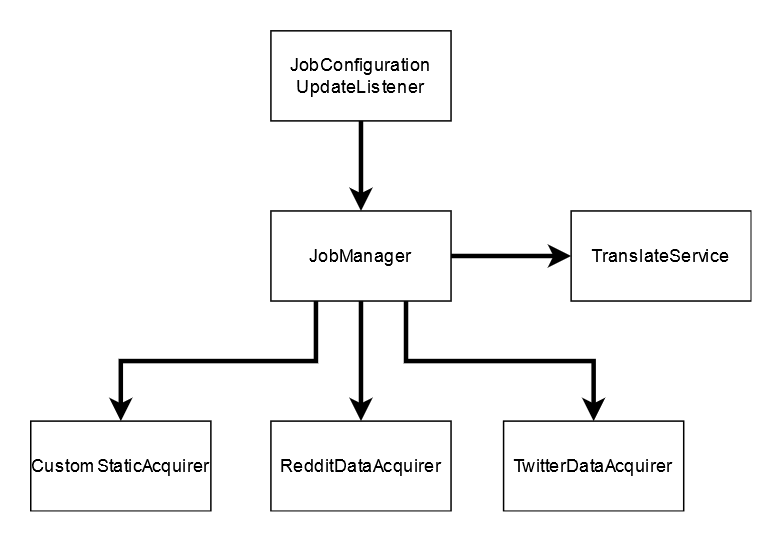
\includegraphics[width=0.8\textwidth]{diagrams/class-da.png}
    \caption{Relationships among major classes of Data acquirer}
    \label{figure:class-da}
\end{figure}

\subsection{Configuration}\label{subsubsection:acqconfig}

The configuration of an acquirer is stored in the project \texttt{WebApi.*} in the file \texttt{appsettings.json}. It does not require any user input. The configuration is distributed via a dependency injection container. Each option of the configuration needs to be bound to the file. This binding is in the project \texttt{Application} in the file \texttt{DataAcquisitionService\-WebApiBuilder.cs}.

\noindent
The most notable configuration objects are:

\begin{itemize}
    \item \texttt{ComponentOptions} - This object contains identity of the acquirer and Kafka topics which it uses.
    \item \texttt{TranslatorOptions} - This object contains settings of the translator service. Endpoint and subscription key can be found in a Azure Text Translator resource.
    \item \texttt{MinioOptions} - URL and credentials of the Minio server.
\end{itemize}

\subsection{Build + Run}

Navigate to the source code, specifically to the \texttt{acquisition/DataAcquirer/Web.*} and type in the following commands:

\begin{itemize}
    \item \texttt{dotnet restore} - downloads all third party libraries
    \item \texttt{dotnet build} - build the projects
    \item \texttt{dotnet run} - run the projects
\end{itemize}

\subsection{Communication}\label{subsection:da_communication}

JMS uses Kafka for the communication depicted in Figure \ref{fig:apiDa}

\begin{figure}[H]
    \centering
    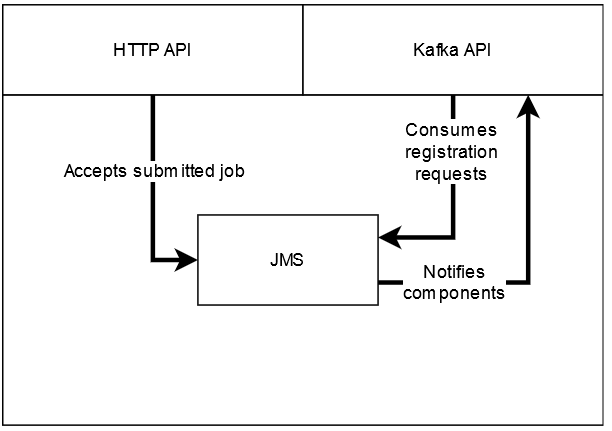
\includegraphics[width=0.8\textwidth]{diagrams/api-jms.png}
    \caption{Kafka interface is used to listen to job notification, produce posts and register the component}
    \label{fig:apiDa}
\end{figure}

\subsubsection{Kafka Interface}\label{subsubsection:da_kafkainterface}

Data acquirers listens for two types of job notification (see Appendix \ref{subsection:notification}): start job and stop job.

The start job notification has the following fields:

\begin{itemize}
    \item \texttt{jobId} - Id of the job
    \item \texttt{command} - In case of start job, it is always \texttt{START}
    \item \texttt{attributes} - attributes of the acquirer. It is discussed in more detail below.
    \item \texttt{outputChannelNames} - An array of topics that the acquirer produce posts into.
\end{itemize}

NOTE: The start notification is the same for analysers too.  
\\

Each acquirer requires different attributes:

\paragraph{Twitter Data Acquirer:}
\begin{itemize}
    \item \texttt{TopicQuery} - name of the topic
    \item \texttt{Translate} - is \texttt{"true"} when the post should be translated
    \item \texttt{ApiKey} - Api key used to identify application to the Twitter API.
    \item \texttt{ApiSecretKey} - Api secret  used to authenticate the application
    \item \texttt{AccessToken} - Access token issued by twitter application.
    \item \texttt{AccessTokenSecret} - Acess token secret used for authentication.
\end{itemize}{}

Example: 
\begin{lstlisting}[language=json,firstnumber=1]
{
  ...
  "attributes": {
    "TopicQuery":"weather pocasi",
    "Translate":"true",
    "ApiKey":"123erbs",
    "ApiSecret":"sdsfabnakaler"
    "AccessToken":"assadfsa23234dafadsfn1234123",
    "AccessTokenSecret":"ghfgdr4350234daf"
    }
}
\end{lstlisting}
The credentials showed do not represent valid credentials.

\paragraph{Reddit Data Acquirer}
\begin{itemize}
    \item \texttt{TopicQuery} - name of the topic
    \item \texttt{Translate} - is \texttt{"true"} when the post should be translated
    \item \texttt{appId} - Id of the application registered with twitter
    \item \texttt{appSecret} - Secret used to authorize the application.
    \item \texttt{refreshToken} - Token which is used to not let the session expire.
\end{itemize}{}

Example: 
\begin{lstlisting}[language=json,firstnumber=1]
{
  ...
  "attributes": {
    "TopicQuery":"weather;pocasi",
    "Translate":"true",
    "appId":"mffSocnetoApp",
    "appSecret":"adf289e8lmfals",
    "refreshToken":"klfoiowen1231"
    }
}
\end{lstlisting}
The credentials showed do not represent valid credentials.

\paragraph{Custom Static Data Acquirer:}
\begin{itemize}
    \item \texttt{Translate} - is \texttt{"true"} when the post should be translated
    \item \texttt{bucketName} - Name of the bucket in which is the custom data stored.
    \item \texttt{objectName} - Name of the dataset file
    \item \texttt{mappingName} - Name of the file with mapping
    
\end{itemize}{}

Example: 
\begin{lstlisting}[language=json,firstnumber=1]
{
  ...
  "attributes": {
    "Translate":"true",
    "bucketName":"example-dataset",
    "objectName":"myData.json",
    "mappingName":"myData.mapping"
    }
}
\end{lstlisting}

The stop job notification has the following fields:

\begin{itemize}
    \item \texttt{jobId} - Id of the job
    \item \texttt{command} - In case of stop job, it is always \texttt{Stop}
\end{itemize}

\subsubsection{Outgoing Communication}\label{section:da_outgoing}

\paragraph{Registration}
Acquirer needs to register itself on startup. The registration request was already discussed in the section JMS subsection Outgoing communication (see Section  \ref{subsubsection:jms_kafkainterface}).

\paragraph{Posts}

Data acquirer produces posts (see Appendix \ref{subsection:postmessage})  with the following fields:

\begin{itemize}
    \item \texttt{id} - Guid of the post
    \item \texttt{originalId} - Original id of the post issued by the respective social network.
    \item \texttt{jobId} - Id of the job in which context this post was produced
    \item \texttt{text} - Text of the post.
    \item \texttt{originalText} - If the translation is activated and the post was not originally in English, this field contains the original text and the field \texttt{text} contains the translation.
    \item \texttt{authorId} - Id of the author. In case of anonymous author,  value "0" is used.
    \item \texttt{language} - Language of the post in ISO 639-1 format.
    \item \texttt{datetime} - Datetime when to post was created conforming to format \texttt{YYYY-mm-DDTHH:MM:SS}.
\end{itemize}

The posts are typically produced to two channels: one that is consumed by the storage and the other consumed by all analysers since analysers produce only analyses, not the posts. These two entities are joined in the storage. Names of the channels are configurable and are discussed in the configuration part of Data acquirer (Section \ref{subsubsection:acqconfig}).
